\section{Tokenization and Failure}

For both \texttt{o200k\_base} and DistilBERT WordPiece, we compare clean and attacked token sequences using relative token-count change, normalized token edit distance, and multiset Jaccard overlap. The principal association model is a binomial regression restricted to clean-correct, effectively changed examples:
\begin{equation}
\mathrm{logit}\,P(\mathrm{failure}) = \beta_0 + \beta_1 d_{\mathrm{tok}} + \beta_2 \Delta n + \mathbf{c},
\end{equation}
where $\mathbf{c}$ controls for dataset, attack family, strength, and model seed when applicable. Standard errors are clustered by original example because each input appears under repeated perturbations. Coefficients are interpreted as associations, not causal effects.

The association is large for both subword systems. For BPE features, a one-standard-deviation increase in normalized token edit distance corresponds to 2.64 times the odds of failure (95\% CI 2.46--2.82). For DistilBERT WordPiece the odds ratio is 3.61 (3.38--3.85). Relative token-count change remains positively associated with BPE failure (OR 1.25, 1.19--1.32) after controlling for edit distance, but its DistilBERT coefficient is slightly negative (OR 0.94, 0.91--0.97). This sign difference cautions against using token count alone as a robustness proxy: the identity and ordering of replacement tokens contain information not captured by length.

Figure~\ref{fig:tokenization} provides a nonparametric view. Failure rates rise across token-edit quartiles for both datasets and systems, consistent with the regression. The analysis is restricted to clean-correct examples with at least one effective code-point change, so it models attack failure rather than conflating it with baseline errors. Nevertheless, the result is associational. Attack families jointly determine both token disruption and difficulty, and the controls cannot establish that tokenization changes themselves cause each error.

\begin{figure}[t]
  \centering
  \IfFileExists{../artifacts/figures/token_disruption_failure.pdf}{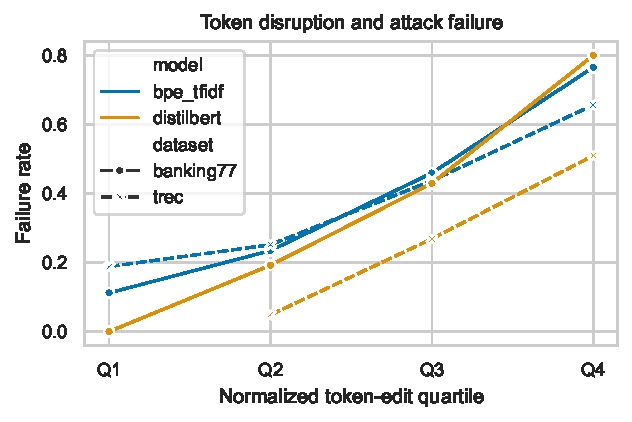
\includegraphics[width=\columnwidth]{token_disruption_failure.pdf}}{\fbox{Tokenization figure pending.}}
  \caption{Failure rate by token-sequence disruption quartile.}
  \label{fig:tokenization}
\end{figure}
